\documentclass[11pt]{article}
% Shared preamble for the notes in this repository. pdfLaTeX, TeX Live 2024 or later.
\usepackage[a4paper,margin=2.6cm]{geometry}
\usepackage[T1]{fontenc}
\usepackage{lmodern}
\usepackage{microtype}
\usepackage{amsmath,amssymb,amsthm}
\usepackage{graphicx}
\usepackage{booktabs}
\usepackage{enumitem}
\usepackage[dvipsnames]{xcolor}
\usepackage[hidelinks]{hyperref}
\hypersetup{colorlinks=true,linkcolor=MidnightBlue,citecolor=MidnightBlue,urlcolor=MidnightBlue}
\graphicspath{{../../figures/}}
\setlist{itemsep=2pt,topsep=4pt}

\newtheorem{theorem}{Theorem}
\newtheorem{proposition}[theorem]{Proposition}
\newtheorem{corollary}[theorem]{Corollary}
\newtheorem{conjecture}[theorem]{Conjecture}
\theoremstyle{definition}
\newtheorem{definition}[theorem]{Definition}
% Reusable derivations, numbered note.k; each note sets \notenumber. Indexed in DERIVATIONS.md.
\newcommand{\notenumber}{0}
\newtheorem{derivation}{Derivation}
\renewcommand{\thederivation}{\notenumber.\arabic{derivation}}
\newtheorem{question}{Question}
\theoremstyle{remark}
\newtheorem{remark}[theorem]{Remark}

\newcommand{\Z}{\mathbb{Z}}
\newcommand{\Q}{\mathbb{Q}}
\newcommand{\R}{\mathbb{R}}
\newcommand{\C}{\mathbb{C}}
\newcommand{\HH}{\mathbb{H}}
\newcommand{\SL}{\mathrm{SL}}
\newcommand{\Gal}{\mathrm{Gal}}
\newcommand{\Hom}{\mathrm{Hom}}
\newcommand{\repo}{\href{https://github.com/rmorleysmith/l-functions-and-physics}{\texttt{l-functions-and-physics}}}
\newcommand{\formal}{\href{https://github.com/rmorleysmith/morley-smith-formal}{\texttt{morley-smith-formal}}}
\newcommand{\script}[1]{\href{https://github.com/rmorleysmith/l-functions-and-physics/blob/main/scripts/#1}{\texttt{scripts/#1}}}
% A path inside the Lean repository; it may break after a slash.
\newcommand{\leanpath}[1]{\nolinkurl{#1}}

% Grades used in every status table.
\newcommand{\gradeLean}{\textsc{lean}}      % proved in Lean 4 with Mathlib
\newcommand{\gradeClassical}{\textsc{classical}}  % a published theorem, cited
\newcommand{\gradeComputed}{\textsc{computed}}    % checked numerically by a script in this repository
\newcommand{\gradeConvention}{\textsc{convention}}  % a choice of units or names
\newcommand{\gradeOpen}{\textsc{open}}      % a question, conjecture or working hypothesis
% The legend printed under every status table.
\newcommand{\gradelegend}{\par\nopagebreak\smallskip\noindent\begin{minipage}{\textwidth}\small
\gradeLean: proved in Lean 4 with Mathlib.
\gradeClassical: a published theorem.
\gradeComputed: checked numerically by a script in the repository \repo.
\gradeConvention: a choice of units or names.
\gradeOpen: a question, conjecture or working hypothesis.
\end{minipage}\par\medskip}
% A plain-language physical reading, placed after each derivation.
\newcommand{\physical}{\paragraph{In physical terms.}}

\renewcommand{\notenumber}{7}

\title{Impulses, packets and spectra}
\author{Richard Morley-Smith}
\date{Note 07 \quad November 2026}

\begin{document}
\maketitle

\begin{abstract}
\noindent
Treat the primes as a train of unit impulses: one click at each prime power $p^k$, of strength $\log p$.
Five reusable derivations turn this train into orthogonal packets and a continuous spectrum, and back.
\begin{itemize}
\item Poisson summation pairs a comb of impulses with a comb of waves.
\item The character table modulo 12 is a Hadamard matrix, so the train splits into four orthogonal packets, the residue classes $1,5,7,11$, with energy conserved.
\item The Laplace transform of each packet is $-L'/L$ of a Dirichlet $L$-function.
\item The explicit formula rebuilds each packet from the zeros of the $L$-functions.
\item Conversely, the zeros, read as frequencies, ring at the logarithms of the prime powers (Landau).
\end{itemize}
Primes and zeros are a Fourier pair.
Chebyshev's bias, the lag of the class $1 \bmod 12$, is an imbalance between packets.
Every statement is checked numerically.
\end{abstract}

\section{The picture}

Record a click at each time $u = \log 2, \log 3, \log 4, \log 5, \log 7,\dots$, the logarithms of the prime powers, with loudness $\log p$.
Three instruments analyse the recording.
\begin{itemize}
\item A \emph{prism}, the characters, splits the clicks into four orthogonal channels without loss.
\item A \emph{transfer function}, the $L$-function, describes each channel's response at every complex frequency $s$.
\item A \emph{spectrum analyser}, the explicit formula, finds that each channel is a sum of pure tones.
\end{itemize}
The tones' frequencies are the zeros of the $L$-functions.
The derivations below make each step exact.

\section{Impulses and waves}

\begin{derivation}[Poisson summation]\label{d:poisson}
For a rapidly decreasing $f$ with Fourier transform $\hat f(\xi) = \int f(x)e^{-2\pi i x\xi}\,dx$,
\[
  \sum_{n\in\Z} f(n) = \sum_{k\in\Z}\hat f(k).
\]
For $f(x) = e^{-\pi x^2 t}$ this gives $\theta(1/t) = \sqrt t\,\theta(t)$, where $\theta(t) = \sum_n e^{-\pi n^2 t}$.
\end{derivation}

\noindent
The proof: the periodic function $\sum_n f(x+n)$ has Fourier coefficients $\hat f(k)$, so evaluate its Fourier series at $x=0$.
\physical A comb of unit impulses, blurred by diffusion for a time $t$, is the same as its comb of frequencies blurred for time $1/t$.
The same derivation, in two dimensions, gives the modularity of the lattice theta series of note~02.
Checked at $t = 0.37$ and $1.9$ by \script{impulses\_packets.py}.

\section{Orthogonal packets}

\begin{derivation}[the prism]\label{d:prism}
The four characters modulo 12 take the values below on the classes $a = 1,5,7,11$.
The matrix $H$ satisfies $HH^{\mathsf T} = 4I$; it is a Hadamard matrix.
\[
  H = \begin{pmatrix} 1&1&1&1\\ 1&1&-1&-1\\ 1&-1&1&-1\\ 1&-1&-1&1\end{pmatrix}
  \quad(\text{rows } \chi_0,\ \chi_{-4},\ \chi_{-3},\ \chi_{12}).
\]
Hence, for $n$ coprime to 12, $\mathbf 1[n\equiv a] = \tfrac14\sum_\chi\chi(a)\chi(n)$.
For the impulse trains $\psi(x;12,a) = \sum_{n\le x,\,n\equiv a}\Lambda(n)$ and $\psi(x,\chi) = \sum_{n\le x}\chi(n)\Lambda(n)$,
\[
  \psi(x;12,a) = \tfrac14\sum_\chi\chi(a)\,\psi(x,\chi),\qquad \sum_a\psi(x;12,a)^2 = \tfrac14\sum_\chi\psi(x,\chi)^2.
\]
\end{derivation}

\physical The four packets are orthogonal channels.
Splitting the impulses into residue classes and recombining them by characters loses nothing, and the total energy (sum of squares) is the same in both descriptions, as for light split into orthogonal polarisations.
The script checks both identities exactly at $x = 10^2, 10^4, 10^6$ (Figure~\ref{fig:packets}).

\begin{figure}[ht]
  \centering
  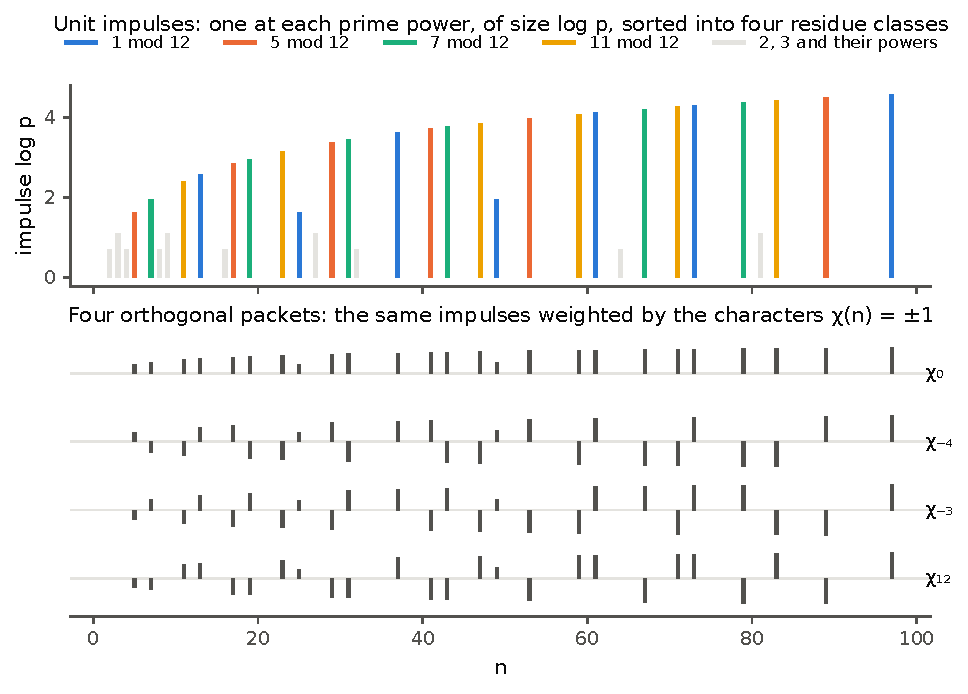
\includegraphics[width=0.9\textwidth]{imp-packets}
  \caption{Top: the impulse train up to 100, coloured by residue class modulo 12. Bottom: the same impulses weighted by the four characters.}
  \label{fig:packets}
\end{figure}

\section{The $L$-function is the transform of a packet}

\begin{derivation}[transfer function]\label{d:transfer}
For $\mathrm{Re}\,s>1$,
\[
  -\frac{L'}{L}(s,\chi) = \sum_{n\ge1}\frac{\chi(n)\Lambda(n)}{n^s} = \int_0^\infty e^{-su}\,d\psi_\chi(e^u).
\]
\end{derivation}

\noindent
The proof: take logarithms of the Euler product, $\log L(s,\chi) = \sum_p\sum_k\chi(p)^kp^{-ks}/k$, and differentiate.
\physical In the variable $u=\log x$, the right side is the Laplace transform of the impulse train.
So the $L$-function is the transfer function of the packet, its response at complex frequency $s$.
Its poles (the zeros of $L$) are the packet's resonances.
The script compares the sum over $n\le10^6$ with $-L'/L(2,\chi)$ for $\chi_{-4},\chi_{-3},\chi_{12}$; they agree to $5\times10^{-5}$.

\section{The explicit formula: packets from zeros}

\begin{derivation}[explicit formula]\label{d:explicit}
Invert Derivation~\ref{d:transfer} (Perron's formula) and collect residues.
For $x>1$ not a prime power,
\[
  \psi(x) = x - \sum_\rho\frac{x^\rho}{\rho} - \log 2\pi - \tfrac12\log(1-x^{-2}),
\]
and for a primitive character $\chi$ of parity $a$,
\[
  \psi(x,\chi) = -\sum_\rho\frac{x^\rho}{\rho} - (1-a)\log x - b(\chi) + \sum_{m\ge1}\frac{x^{a-2m}}{2m-a}.
\]
The constant is $b(\chi) = L'(0,\chi)/L(0,\chi)$ if $a=1$, and $\lim_{s\to0}\big(L'/L(s,\chi)-1/s\big)$ if $a=0$.
The sums run over the non-trivial zeros, taken symmetrically \cite{Davenport}.
\end{derivation}

\noindent
A zero $\rho = \tfrac12+i\gamma$ and its conjugate together contribute $-2\,\mathrm{Re}\,(x^\rho/\rho)$.
As a function of $u = \log x$, that is a pure tone of frequency $\gamma$ with amplitude $2e^{u/2}/|\rho|$.
\physical Each zero is a normal mode of the impulse train, and the train is the sum of its modes.
The pole at $s=1$ gives the smooth part $x$.

The script finds every zero below height 150 by the sign changes of Hardy's $Z$ (note~04).
There are 52, 85, 78 and 111 zeros for $\zeta$, $\chi_{-4}$, $\chi_{-3}$ and $\chi_{12}$, against Riemann--von Mangoldt main terms of $52.7$, $85.0$, $78.1$ and $111.2$.
It then rebuilds the four packets $\psi(x;12,a)$ by Derivations~\ref{d:prism} and~\ref{d:explicit}, after removing the impulses at the powers of 2 and 3 from the primitive characters.
The root-mean-square error on $3<x<150$ falls from $0.83$ to $0.53$ to $0.42$ as the height grows from 50 to 100 to 150 (Figure~\ref{fig:explicit}).
The rebuild uses the zeros found on the critical line, as the generalised Riemann hypothesis predicts.

\begin{figure}[ht]
  \centering
  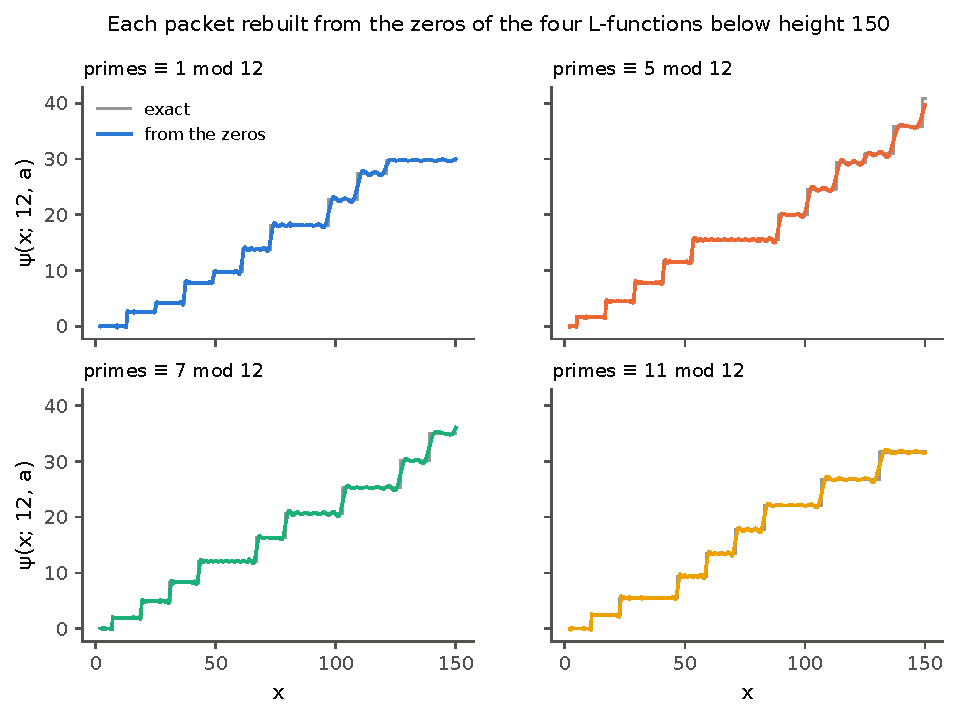
\includegraphics[width=0.9\textwidth]{imp-explicit}
  \caption{The four packets, exact (grey steps) and rebuilt from the zeros below height 150 of the four $L$-functions (colour).}
  \label{fig:explicit}
\end{figure}

\section{The spectrum of the zeros}

\begin{derivation}[Landau's formula]\label{d:landau}
For fixed $x>1$, as $T\to\infty$,
\[
  \sum_{0<\gamma\le T} x^{i\gamma} = -\frac{T}{2\pi}\,\frac{\Lambda(x)}{\sqrt x} + O(\log T),
\]
where $\Lambda(x)=0$ unless $x$ is a prime power \cite{Landau}.
\end{derivation}

\physical Read the zeros as the lines of a spectrum, and play them all at once.
The result is silent except at $u = \log p^k$, where it rings with depth proportional to $\Lambda(p^k)/p^{k/2}$.
The zeros behave like a crystal whose diffraction pattern has its Bragg peaks at the logarithms of the prime powers.
Dyson suggested reading the zeros as a one-dimensional quasicrystal for this reason \cite{Dyson}.
With the first 600 zeros of $\zeta$ ($T = 939.02$), the script finds $\sum\cos(\gamma\log x) = -73.3$, $-93.3$, $-50.6$, $-107.3$ and $-108.7$ at $x = 2, 3, 4, 5, 7$.
Landau's main term predicts $-73.2$, $-94.8$, $-51.8$, $-107.6$ and $-109.9$.
Every deep dip of the smoothed spectrum on $0.3<u<3.3$ sits at a prime power (Figure~\ref{fig:landau}).
Together with Derivation~\ref{d:explicit}, this is the sense in which primes and zeros are a Fourier pair.
Note~04 showed the primes as tones in $t$, with frequencies $\log p$; here the zeros are tones in $u$, with frequencies $\gamma$.

\begin{figure}[ht]
  \centering
  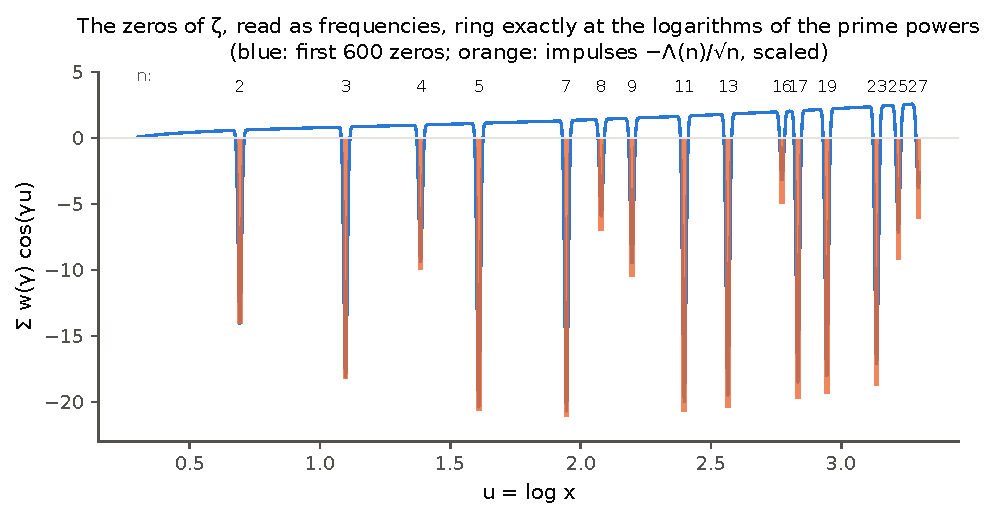
\includegraphics[width=0.9\textwidth]{imp-landau}
  \caption{The first 600 zeros of $\zeta$ as frequencies, with a Gaussian taper (blue), against the impulses $-\Lambda(n)/\sqrt n$, scaled to match at $n=2$ (orange).}
  \label{fig:landau}
\end{figure}

\section{An imbalance between packets: Chebyshev's bias}

Counting primes rather than prime powers, the four classes fill unevenly.
Up to $10^6$ there are $19564$, $19611$, $19667$ and $19654$ primes in the classes $1,5,7,11$, and the class $1$ is the emptiest.
Its deficit grows like a slow drift (Figure~\ref{fig:bias}).
\physical Every prime square is $\equiv 1 \pmod{12}$.
The full impulse train $\psi$ includes the squares, and its packets are balanced to leading order.
Remove the squares, as counting primes does, and the class of the squares is the one that comes up short.
Rubinstein and Sarnak made this precise, under the generalised Riemann hypothesis and a linear-independence hypothesis on the zeros \cite{RubinsteinSarnak}.

\begin{figure}[ht]
  \centering
  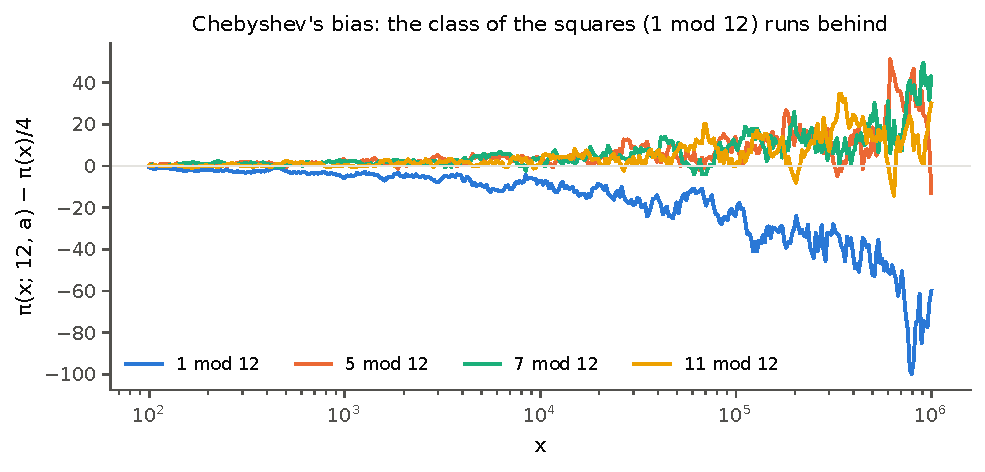
\includegraphics[width=0.9\textwidth]{imp-bias}
  \caption{$\pi(x;12,a) - \pi(x)/4$ for the four classes, $10^2\le x\le10^6$.}
  \label{fig:bias}
\end{figure}

\section*{Status of the statements}

\begin{center}
\small
\begin{tabular}{@{}p{0.62\textwidth}l@{}}
\toprule
Statement & Grade\\
\midrule
Derivations~\ref{d:poisson}--\ref{d:landau} & \gradeClassical\\
$HH^{\mathsf T}=4I$; packet split and Parseval at $10^2,10^4,10^6$ & \gradeComputed\\
$-L'/L(2,\chi)$ from the impulses; zero counts; rebuild errors & \gradeComputed\\
Landau's formula at $x = 2,3,4,5,7$; dips at prime powers & \gradeComputed\\
Chebyshev's bias at $10^6$ & \gradeComputed; theory \gradeClassical{} (conditional)\\
All zeros on the critical line (GRH) & \gradeOpen\\
\bottomrule
\end{tabular}
\end{center}

\begin{thebibliography}{9}
\bibitem{Davenport} H.~Davenport, \emph{Multiplicative Number Theory}, 3rd ed., Springer, 2000.
\bibitem{Dyson} F.~Dyson, Birds and frogs, \emph{Notices Amer. Math. Soc.} 56 (2009), 212--223.
\bibitem{Landau} E.~Landau, \"Uber die Nullstellen der Zetafunktion, \emph{Math. Ann.} 71 (1912), 548--564.
\bibitem{RubinsteinSarnak} M.~Rubinstein and P.~Sarnak, Chebyshev's bias, \emph{Experiment. Math.} 3 (1994), 173--197.
\end{thebibliography}

\end{document}
